The rule engine decides which rules may need to be executed while respecting the
rule priority semantics presented in Section~\ref{sec:language:semantics}. The
rule engine is composed of 3 data structures:

\begin{itemize}

   \item \emph{Rule Queue} is a bitmap representing the rules currently
      scheduled to run. When bit $i$ in the \emph{Rule Queue} is set, it
      means that rule $i$ is scheduled to be run. A rule $i$ is set to run
      when all the facts that satisfy the rule's LHS are available.
      Rules are executed by fetching the least significant bit of
      the bitmap, unsetting that bit and then executing the corresponding rule.
      This operation is accomplished by using the \emph{bit scan forward (bsf)}
      assembly instruction available on x86/x86-64 machines;

   \item \emph{Rule Counter} counts the number of predicates that exist in the
      database and that are needed by a rule. For instance, the rule \code{a,
      e(1) -o b} needs predicates \code{a} and \code{e}, which means that when
      the count in the rule counter goes up to two, then the rule is scheduled
      to run. Likewise, if the counter is decremented to one then the rule is
      removed from the \emph{Rule Queue}.

   \item \emph{Predicate Bitmap} is a bitmap representing the existence of facts
      for a given predicate in the database. When a predicate becomes available
      then the \emph{Rule Counter} is updated to take into account the existence
      of new facts.

\end{itemize}


\begin{figure}[t]
   \begin{center}
\begin{BVerbatim}[numbers=left,fontsize=\codesize]
a, e(1) -o b.  // Rule 1.
a -o c.        // Rule 2.
b -o d.        // Rule 3.
e(0) -o f.     // Rule 4.
c -o e(1).     // Rule 5.

a.
e(0).
\end{BVerbatim}
\end{center}
\vspace{5mm}
   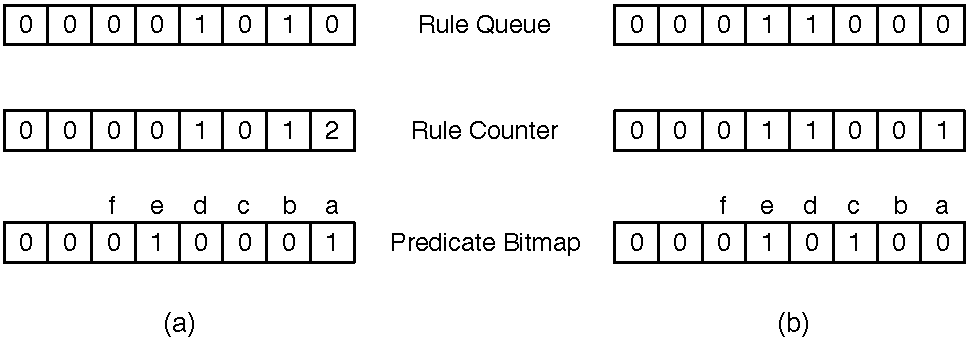
\includegraphics[width=0.96\textwidth]{figures/implementation/rule_queue.pdf}

   \mycap{Example program and corresponding rule engine data structures. The
      initial state is represented in (a), where the rules scheduled to run are
      1, 2 and 4. After attempting rule 1, bit 0 is unset from the \emph{Rule
      Queue}, resulting in (b). Figure (c) is the result of applying rule 2,
      \code{a -o c}, which marks rule 5 in the \emph{Rule Queue} since the rule
      is now \emph{available} in the \emph{Rule Counter}.}

   \label{fig:implementation:rule_engine}
\end{figure}

To better understand how our rule engine works,
Fig.~\ref{fig:implementation:rule_engine} shows an example program and the
corresponding rule engine data structures. When the program starts, the facts
for predicates \code{a} and \code{e} exist, therefore the \emph{Rule Counter}
starts with rules 1, 2 and 4 where the values are 2, 1, and 1, respectively.
Since these rules have the required counter to be applied, the \emph{Rule Queue}
bitmap starts with the same three rules
(Fig.~\ref{fig:implementation:rule_engine}(a)).  In order to pick rules for
execution, we take the rule corresponding to the least significant bit from the
\emph{Rule Queue} bitmap, initially the first rule \code{a, e(1) -o b}.
However, since we don't have fact \code{e(1)}, this rule fails and its bit in
\emph{Rule Queue} must be set to 0.
Figure~\ref{fig:implementation:rule_engine}(b) shows the rule engine data
structures at that point.

The next rule in \emph{Rule Queue} is the second rule \code{a -o c}.  Because
this rule succeeds, fact \code{a} is consumed and fact \code{c} is derived.  We
thus update \code{Predicates Bitmap} accordingly, and decrease the counters for
the first and second rules in \emph{Rule Counter} since such rules are no longer
applicable (\code{a} was consumed), and increase the counter for the fifth rule
since \code{c} was derived. Finally, to update the \emph{Rule Queue}, we must
schedule the fifth rule since its counter has been increased to the required
number (we have all predicates).  Figure~\ref{fig:implementation:rule_engine}(b)
shows the rule engine data structures at that point.  In the continuation, the
rule engine will schedule the fourth and fifth rules to run.

Note that every node in the program requires the set of data structures
presented in Fig.~\ref{fig:implementation:rule_engine}. We use 64 bit integers
to implement the 2 bitmaps and an array of 16 bits integers for the \emph{Rule
Counter}.

For persistent facts, we do a small optimization to reduce the number of
derivations. We divide the program rules into two sets: \emph{persistent rules}
and \emph{non persistent rules}. Persistent rules are rules where only
persistent facts are involved. We compile such rules incrementally, i.e., we
attempt to fire all rules when a new persistent fact is derived. This is called
the \emph{pipelined semi-naive} evaluation and it originated in the P2
system~\cite{Loo-condie-garofalakis-p2}. This evaluation method avoids excessive
re-derivations of the same fact. The order of derivation does not matter for
those rules, since only persistent facts are used.

